\begin{frame}{Modelo Discriminador}
    

    El modelo SRGAN (Super Resolution Generative Adversarial Network) fue
    propuesto en 2016 por un grupo de investigadores de la empresa Twitter.
    La principal innovación de este modelo es su función de pérdida, llamada
    función de pérdida perceptual, que permite mejorar el realismo de la imagen de
    salida.

        
    \begin{figure}[H]
        \begin{center}
          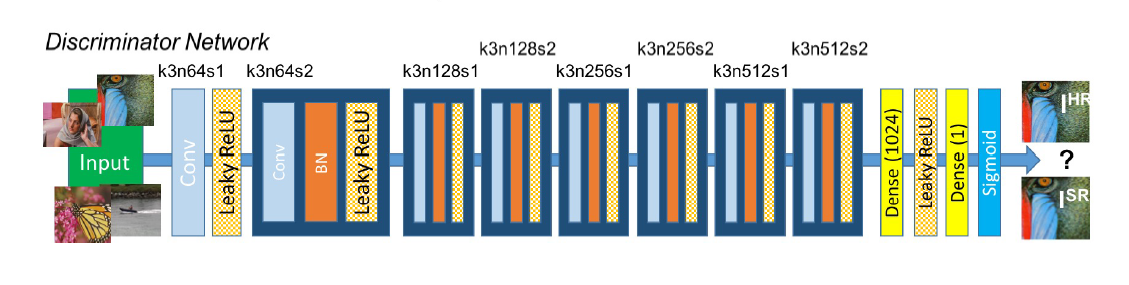
\includegraphics[scale = 0.5]{Imp_discriminador.png}
          \caption{Modelo de entrenamiento del discriminador}
          \label{Alexis3}
        \end{center}
    \end{figure}
     

\end{frame}

\begin{frame}{Modelo Generador}
    

    El modelo SRGAN (Super Resolution Generative Adversarial Network) fue
    propuesto en 2016 por un grupo de investigadores de la empresa Twitter.
    La principal innovación de este modelo es su función de pérdida, llamada
    función de pérdida perceptual, que permite mejorar el realismo de la imagen de
    salida.

        
    \begin{figure}[H]
        \begin{center}
          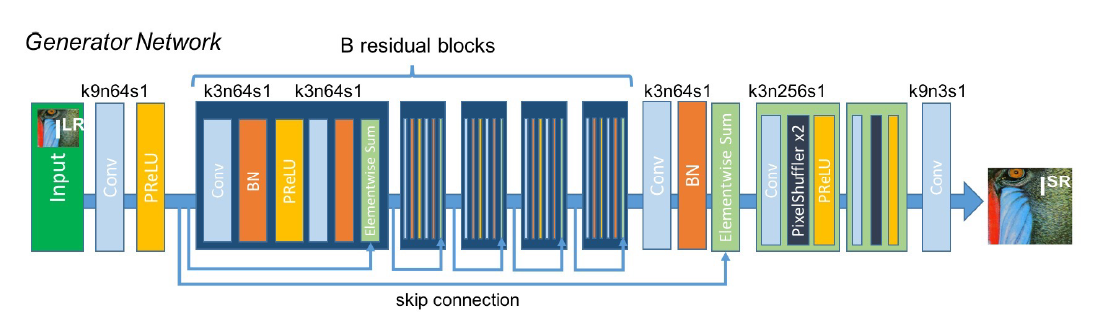
\includegraphics[scale = 0.5]{Imp_generador.png}
          \caption{Modelo de entrenamiento del generador}
          \label{Alexis4}
        \end{center}
    \end{figure}
     

\end{frame}



\begin{frame}{Redes residuales}
    \begin{block}{Bloque Residual}
        hacen la conexión entre capas anteriores con capas futuras (saltos) sin que la información de 
        las características extraídas en capas previas se diluya.
    \end{block}
    \begin{figure}[H]
        \begin{center}
          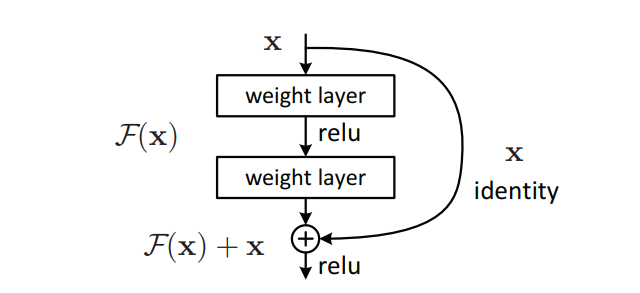
\includegraphics[scale = 0.4]{Residual-Block.png}
          \caption{Funcionamiento del Bloque Residual}
          \label{Alexis10}
        \end{center}
    \end{figure}

\end{frame}


\begin{frame}{Bloques de escalado}
    \begin{figure}[H]
        \begin{center}
          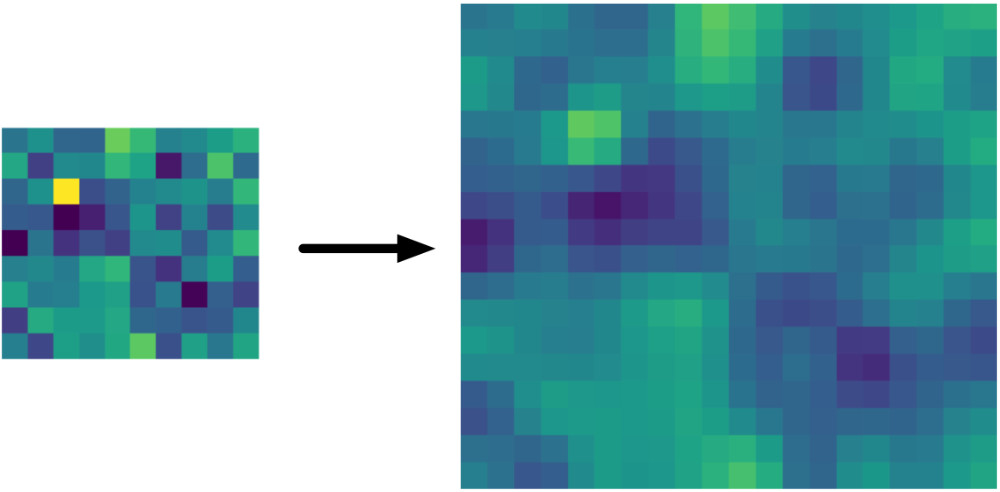
\includegraphics[scale = 0.4]{Bilinear2x.jpg}
          \caption{Red Neuronal Pre-entrenada}
          \label{Alexis5}
        \end{center}
    \end{figure}
     
\end{frame}

\begin{frame}{VGG19}
    
\begin{block}{Red Pre-entrenada}
    Se utiliza una red de entrenamiento pre-entrenada conocida como VGG19
    la cual nos da los pesos necesarios
\end{block}
    \begin{figure}[H]
        \begin{center}
          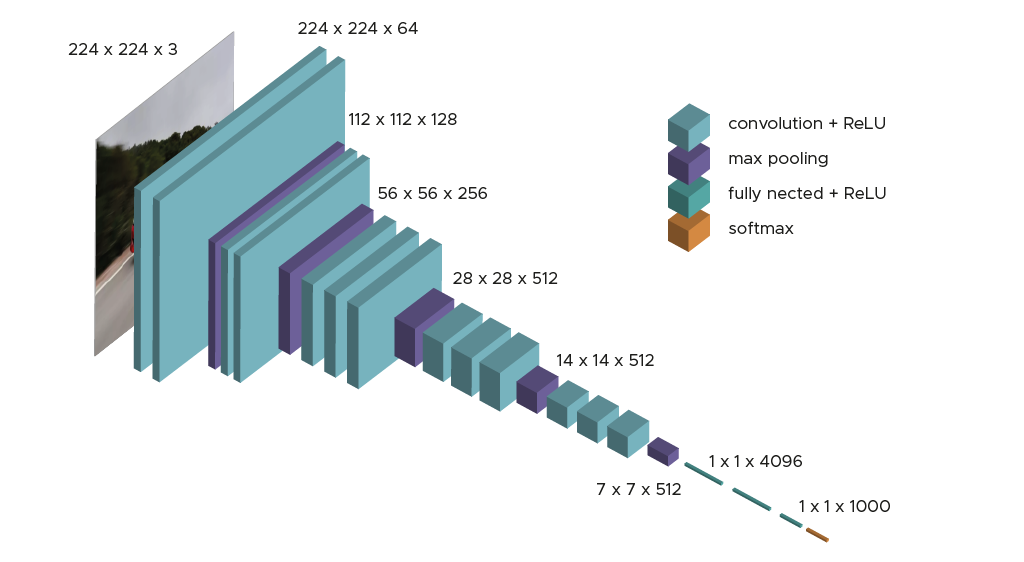
\includegraphics[scale = 0.18]{VGG19.png}
          \caption{Red Neuronal Pre-entrenada}
          \label{Alexis5}
        \end{center}
    \end{figure}
     

\end{frame}


\begin{frame}{Modelos Generadores obtenidos}
    
    \begin{figure}[H]
        \begin{center}
          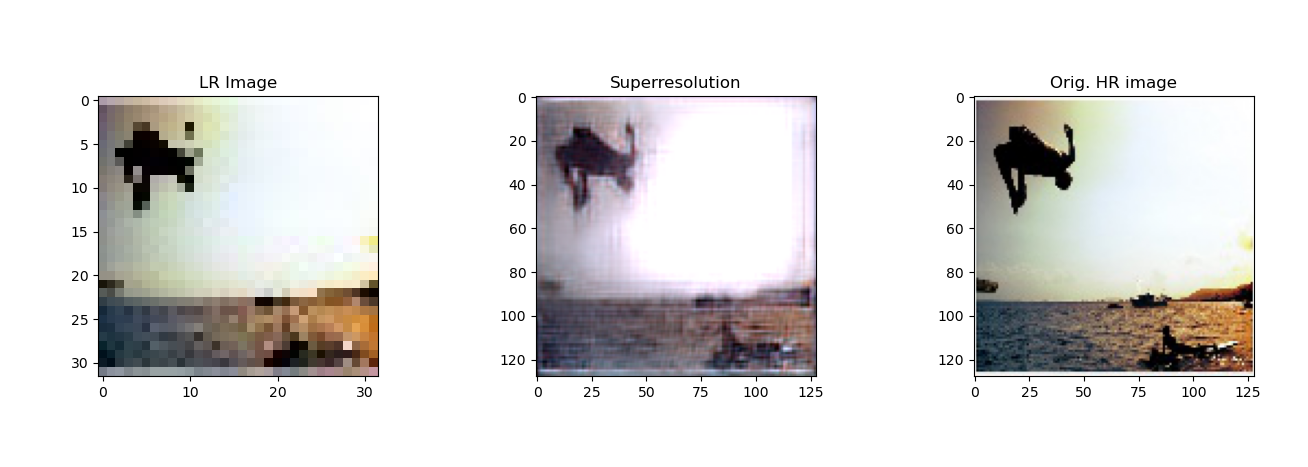
\includegraphics[scale = 0.6]{13im_200E.png}
          \caption{Modelo de entrenamiento del generador}
          \label{Alexis6}
        \end{center}
    \end{figure}
    
\end{frame}

\begin{frame}{Modelos Generadores obtenidos}
    
    \begin{figure}[H]
        \begin{center}
          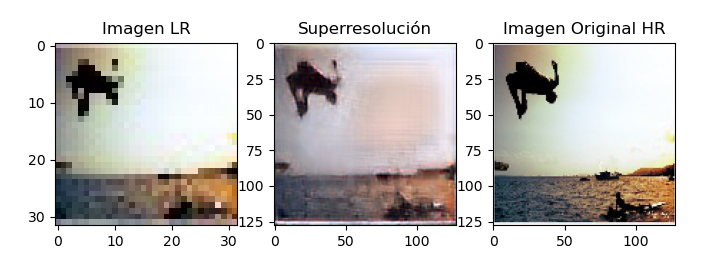
\includegraphics[scale = 0.6]{50im_400E.png}
          \caption{Modelo entrenado con 50 imágenes y 400 épocas}
          \label{Alexis7}
        \end{center}
    \end{figure}
     
\end{frame}


\begin{frame}{Modelos Generadores obtenidos}
    
    \begin{figure}[H]
        \begin{center}
          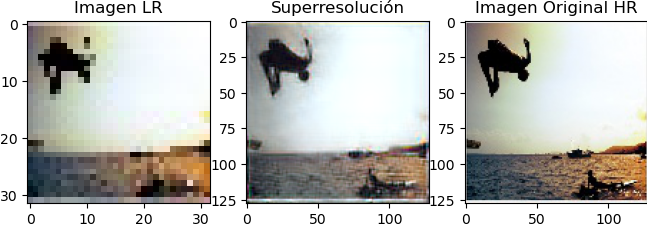
\includegraphics[scale = 0.5]{1000im_5E_Reentrenado.png}
          \caption{Modelo reentrenado 1000 imágenes, 5 épocas}
          \label{Alexis8}
        \end{center}
    \end{figure}
     
\end{frame}

\begin{frame}{Perdidas del modelo}
    
    \begin{figure}[H]
        \begin{center}
          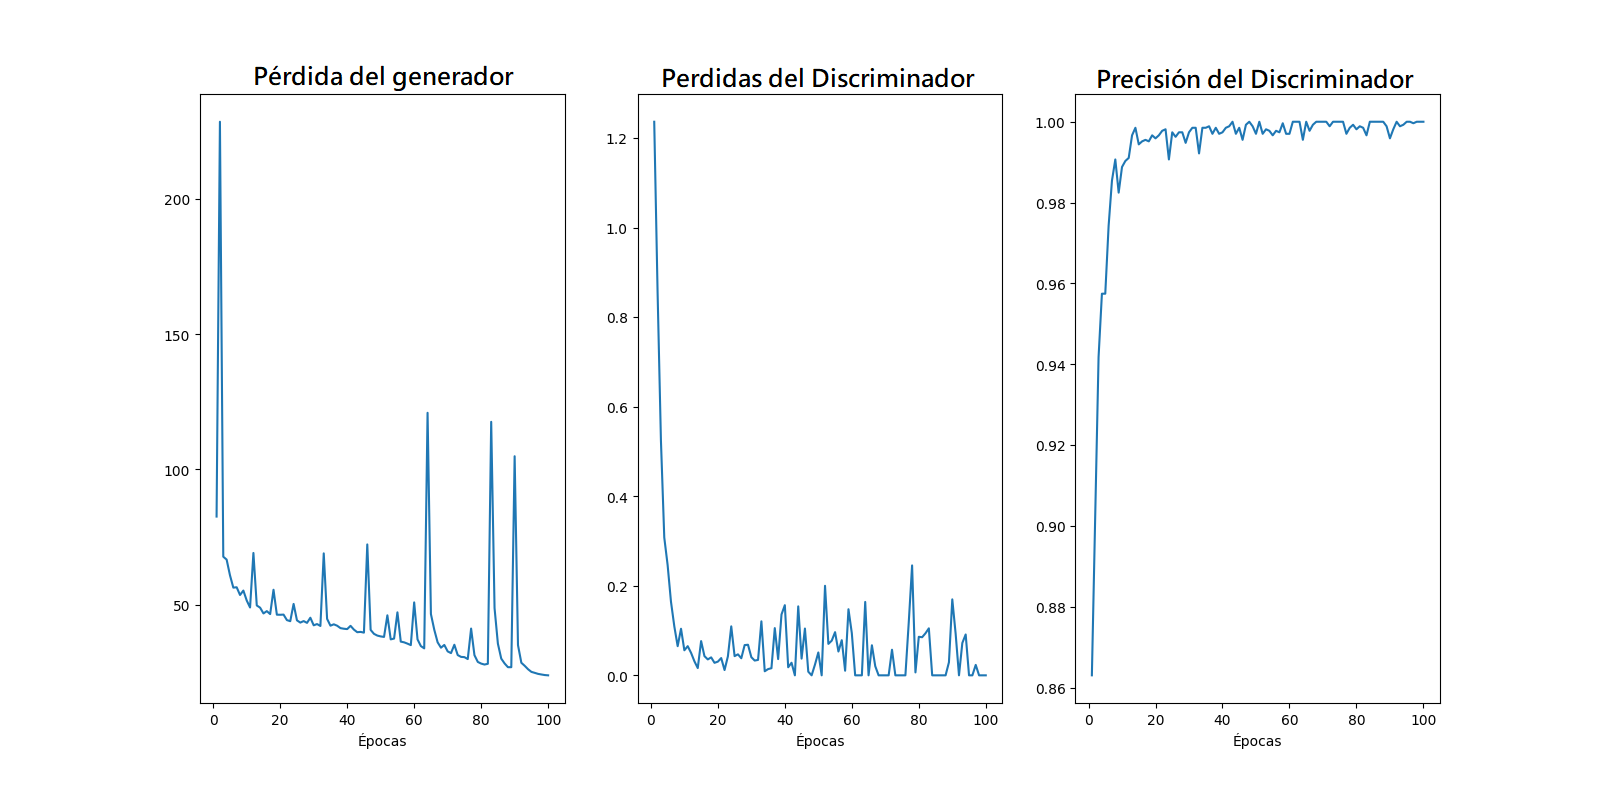
\includegraphics[scale = 0.5]{Graficasperdidas.png}
          \caption{Pérdidas y Precisión del Modelo}
          \label{Alexis8}
        \end{center}
    \end{figure}
     
\end{frame}